% ------------------------------------------------------------------------
% file `1_E_juin-appliquer-16-exercise-body.tex'
%   in folder `xsim/'
%
%     exercise of type `appliquer' with id `16'
%
% generated by the `appliquer' environment of the
%   `xsim' package v0.21 (2022/02/12)
% from source `1_E_juin' on 2024/05/28 on line 400
% ------------------------------------------------------------------------
    Voici un repère cartésien.
    \begin{center}
        
\includegraphics{tikz/repere.tikz}
    \end{center}
    % 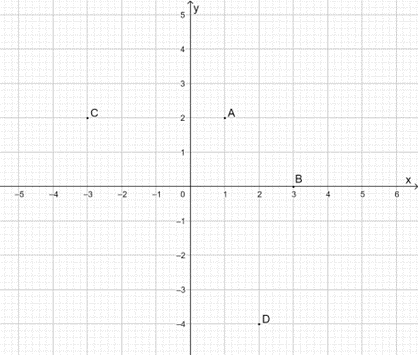
\includegraphics{img/graphe.png}
    \begin{enumerate}
        \item Écris les coordonnées du point \(C\). \\
        \(C(\blank[width=1cm]{}; \blank[width=1cm]{})\)
        \item Place le point \(X\) tel que \(X(-4;-2)\)
        \item Quel est l'abscisse du point \(D\) ? \dotfill
        \item Quelle est l'ordonnée du point \(B\) ? \dotfill
    \end{enumerate}
